% !TEX program = xelatex
\documentclass[notheorems,aspectratio=169]{beamer}

\usepackage{ctex}
\usepackage{fontspec}
\usepackage{xeCJK}
\IfFontExistsTF{Noto Serif CJK JP}{%
  \setCJKmainfont{Noto Serif CJK JP}%
  \setCJKsansfont{Noto Sans CJK JP}%
  \setCJKmonofont{Noto Sans Mono CJK JP}%
}{}
\usepackage{amsmath,amssymb,bm}
\usepackage{booktabs,array}
\usepackage{tikz}
\usetikzlibrary{arrows.meta,angles,quotes,calc,positioning}

\usetheme{Madrid}
\usefonttheme[onlymath]{serif}
\beamertemplatenavigationsymbolsempty
\let\Tiny\tiny

\definecolor{ChinaRed}{RGB}{196,30,58}
\definecolor{JapanBlue}{RGB}{0,82,155}
\definecolor{SoftBlue}{RGB}{231,241,249}
\definecolor{SoftRed}{RGB}{252,235,239}
\definecolor{GraphGray}{RGB}{100,110,120}

\setbeamercolor{structure}{fg=JapanBlue}
\setbeamercolor{alerted text}{fg=ChinaRed}
\setbeamercolor{block title alerted}{bg=ChinaRed,fg=white}
\setbeamercolor{block body alerted}{bg=SoftRed}
\setbeamercolor{block title}{bg=JapanBlue,fg=white}
\setbeamercolor{block body}{bg=SoftBlue}
\setbeamercolor{item projected}{bg=JapanBlue,fg=white}
\setbeamertemplate{itemize item}{\color{JapanBlue}$\blacktriangleright$}
\setbeamertemplate{itemize subitem}{\color{ChinaRed}$\bullet$}

\newtheorem{definition}{定義}
\newtheorem{theorem}{定理}
\newcommand{\jp}[1]{\textbf{\color{JapanBlue}#1}}
\newcommand{\key}[1]{\textbf{\color{ChinaRed}#1}}
\newcommand{\dd}{\mathop{}\!\mathrm{d}}

\title[EJU Physics]{物理1}
\subtitle{位置・変位・速度と運動の合成・分解}
\author[Sirui Liu]{Sirui Liu}
\date{2026年7月18日}

\begin{document}

% 1
\begin{frame}
  \titlepage
\end{frame}

% 2
\begin{frame}{目录}
  \tableofcontents
\end{frame}

\section{位置と変位}

% 3
\begin{frame}{座標系と位置}
  \begin{columns}[T,onlytextwidth]
    \column{0.48\textwidth}
    \begin{block}{位置（Position）}
      物体在哪里，必须先决定\jp{基準点}（reference point）与坐标轴正方向。
      \[
        x=x(t)
      \]
      表示物体的位置随时间变化。
    \end{block}
    \begin{alertblock}{重要}
      “在右边”本身不完整；必须说明\key{相对于哪个原点}。
    \end{alertblock}

    \column{0.48\textwidth}
    \begin{center}
    \begin{tikzpicture}[x=0.68cm,y=0.85cm,>=Latex]
      \draw[->,thick,GraphGray] (-4.3,0)--(4.7,0) node[right]{$x$};
      \foreach \x in {-4,-3,...,4}{\draw (\x,0.12)--(\x,-0.12) node[below]{$\x$};}
      \fill[JapanBlue] (0,0) circle (2.6pt) node[above=6pt]{原点 $O$};
      \fill[ChinaRed] (3,0) circle (3.2pt) node[above=6pt]{物体 $P$};
      \draw[->,very thick,ChinaRed] (0,0.5)--(3,0.5) node[midway,above]{$x=+3\,\mathrm{m}$};
    \end{tikzpicture}
    \end{center}
    \begin{block}{座標系（Coordinate System）}
      原点、单位与正方向共同决定坐标系。
    \end{block}
  \end{columns}
\end{frame}

% 4
\begin{frame}{移動距離と変位}
  \begin{columns}[T,onlytextwidth]
    \column{0.48\textwidth}
    \begin{block}{移動距離（Distance）}
      实际走过路径的\key{总长度}。
      \begin{itemize}
        \item 标量（scalar）
        \item 总是 $0$ 或正数
        \item 与具体路径有关
      \end{itemize}
    \end{block}
    \begin{alertblock}{変位（Displacement）}
      终点位置减去起点位置：
      \[
        \Delta x=x_2-x_1
      \]
      位移有大小和方向。
    \end{alertblock}

    \column{0.48\textwidth}
    \begin{center}
    \begin{tikzpicture}[x=0.95cm,y=0.95cm,>=Latex]
      \coordinate (A) at (0,0);
      \coordinate (B) at (5.2,1.6);
      \draw[very thick,JapanBlue] (A) .. controls (1.2,2.3) and (3.5,-1.0) .. (B);
      \draw[->,ultra thick,ChinaRed] (A)--(B) node[midway,below]{$\Delta\vec r$};
      \fill[black] (A) circle (2.4pt) node[left]{始点};
      \fill[black] (B) circle (2.4pt) node[right]{終点};
      \node[JapanBlue] at (2.6,2.0) {移動距離：曲線の長さ};
      \node[ChinaRed] at (2.8,0.25) {変位：始点から終点へ};
    \end{tikzpicture}
    \end{center}
    \begin{block}{比較}
      距离回答“走了多远”，位移回答“位置改变了多少”。
    \end{block}
  \end{columns}
\end{frame}

% 5
\begin{frame}{変位の正負と往復運動}
  \begin{columns}[T,onlytextwidth]
    \column{0.54\textwidth}
    \begin{center}
    \begin{tikzpicture}[x=0.96cm,y=1cm,>=Latex]
      \draw[->,thick,GraphGray] (-0.5,0)--(7.0,0) node[right]{$x$};
      \foreach \x in {0,1,...,6}{\draw (\x,0.12)--(\x,-0.12) node[below]{$\x$};}
      \fill[JapanBlue] (1,0) circle (2.8pt) node[above=7pt]{$A$};
      \fill[ChinaRed] (5,0) circle (2.8pt) node[above=7pt]{$B$};
      \draw[->,very thick,JapanBlue,bend left=28] (1,0.35) to node[above]{去程 $4\,\mathrm m$} (5,0.35);
      \draw[->,very thick,ChinaRed,bend left=28] (5,-0.35) to node[below]{回程 $4\,\mathrm m$} (1,-0.35);
    \end{tikzpicture}
    \end{center}
    \begin{alertblock}{往復后}
      \[
        \text{移動距離}=8\,\mathrm m,\qquad \Delta x=0
      \]
      回到起点时，位移为零，但移动距离不为零。
    \end{alertblock}

    \column{0.42\textwidth}
    \begin{block}{符号的意义}
      \begin{itemize}
        \item $\Delta x>0$：向正方向改变位置
        \item $\Delta x<0$：向负方向改变位置
        \item $\Delta x=0$：终点与起点相同
      \end{itemize}
    \end{block}
    \key{负号表示方向，不表示“位移很小”。}
  \end{columns}
\end{frame}

\section{速さと速度}

% 6
\begin{frame}{平均の速さ（Average Speed）}
  \begin{definition}
    一段时间内的移动距离除以经过时间：
    \[
      \text{平均の速さ}
      =\frac{\text{移動距離}}{\text{経過時間}}
    \]
  \end{definition}
  \begin{columns}[T,onlytextwidth]
    \column{0.48\textwidth}
    \begin{block}{例}
      物体在 $5\,\mathrm s$ 内移动 $20\,\mathrm m$：
      \[
        \text{平均の速さ}=\frac{20}{5}=4\,\mathrm{m/s}
      \]
    \end{block}
    \column{0.48\textwidth}
    \begin{alertblock}{单位换算}
      \[
        1\,\mathrm{m/s}=3.6\,\mathrm{km/h}
      \]
      因此
      \[
        72\,\mathrm{km/h}=20\,\mathrm{m/s}.
      \]
    \end{alertblock}
  \end{columns}
\end{frame}

% 7
\begin{frame}{平均速度（Average Velocity）}
  \small
  \begin{definition}
    \[
      \bar v=\frac{\Delta x}{\Delta t}
      =\frac{x_2-x_1}{t_2-t_1}
    \]
    平均速度使用\key{位移}，因此带有方向。
  \end{definition}
  \begin{center}
  \renewcommand{\arraystretch}{1.25}
  \begin{tabular}{lccc}
    \toprule
    & 分子 & 方向 & 往返原点时\\
    \midrule
    平均の速さ & 移動距離 & 无 & 通常不为 $0$\\
    平均速度 & 変位 & 有 & 等于 $0$\\
    \bottomrule
  \end{tabular}
  \end{center}
  \begin{alertblock}{例}
    $10\,\mathrm s$ 内向右 $30\,\mathrm m$，再向左 $10\,\mathrm m$：
    \[
      \text{平均の速さ}=4\,\mathrm{m/s},\qquad
      \bar v=+2\,\mathrm{m/s}.
    \]
  \end{alertblock}
\end{frame}

% 8
\begin{frame}{瞬間速度（Instantaneous Velocity）}
  \begin{columns}[T,onlytextwidth]
    \column{0.52\textwidth}
    \begin{block}{平均から瞬間へ}
      时间间隔越来越小时：
      \[
        v(t)=\lim_{\Delta t\to0}\frac{\Delta x}{\Delta t}
        =\frac{\dd x}{\dd t}
      \]
      速度是位置对时间的导数。
    \end{block}
    \begin{alertblock}{物理意义}
      瞬时速度描述物体\key{此刻移动得多快、朝哪个方向}。
    \end{alertblock}

    \column{0.44\textwidth}
    \begin{center}
    \begin{tikzpicture}[x=0.82cm,y=0.82cm,>=Latex]
      \draw[->,GraphGray] (-0.3,0)--(5.4,0) node[right]{$t$};
      \draw[->,GraphGray] (0,-0.2)--(0,4.0) node[above]{$x$};
      \draw[very thick,JapanBlue] (0.2,0.2) .. controls (1.7,0.5) and (3.6,1.8) .. (5.0,3.6);
      \coordinate (P) at (3.25,1.75);
      \fill[ChinaRed] (P) circle (2.6pt) node[above left]{$P$};
      \draw[very thick,ChinaRed] ($(P)+(-1.2,-0.85)$)--($(P)+(1.3,0.93)$) node[right]{接線};
      \node[align=center] at (3.6,0.55) {接线斜率\\$=v(t)$};
    \end{tikzpicture}
    \end{center}
  \end{columns}
\end{frame}

% 9
\begin{frame}{速度の向きと符号}
  \begin{columns}[T,onlytextwidth]
    \column{0.47\textwidth}
    \begin{block}{$v>0$}
      物体向坐标轴的\jp{正方向}运动。
    \end{block}
    \begin{alertblock}{$v<0$}
      物体向坐标轴的\key{负方向}运动。
    \end{alertblock}
    \begin{block}{$v=0$}
      该时刻瞬时静止；之后可能继续运动或改变方向。
    \end{block}

    \column{0.49\textwidth}
    \begin{center}
    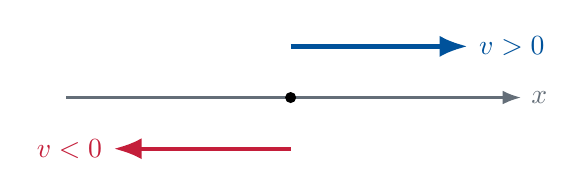
\begin{tikzpicture}[x=0.75cm,y=1cm,>=Latex]
      \draw[->,thick,GraphGray] (-3.8,0)--(3.9,0) node[right]{$x$};
      \fill[black] (0,0) circle (2pt);
      \draw[->,ultra thick,JapanBlue] (0,0.65)--(3.0,0.65) node[right]{$v>0$};
      \draw[->,ultra thick,ChinaRed] (0,-0.65)--(-3.0,-0.65) node[left]{$v<0$};
    \end{tikzpicture}
    \end{center}
    \begin{alertblock}{注意}
      \key{速さ}是 $|v|$。因此速度可为负，速率不能为负。
    \end{alertblock}
  \end{columns}
\end{frame}

\section{運動のグラフ}

% 10
\begin{frame}{位置-時間グラフ}
  \begin{columns}[T,onlytextwidth]
    \column{0.56\textwidth}
    \begin{center}
    \begin{tikzpicture}[x=0.92cm,y=0.68cm,>=Latex]
      \draw[->,GraphGray] (-0.3,0)--(6.2,0) node[right]{$t$};
      \draw[->,GraphGray] (0,-2.0)--(0,4.3) node[above]{$x$};
      \draw[very thick,JapanBlue] (0.4,0.4)--(2.3,3.3) node[midway,left]{$v>0$};
      \draw[very thick,GraphGray] (2.3,3.3)--(3.9,3.3) node[midway,above]{静止};
      \draw[very thick,ChinaRed] (3.9,3.3)--(5.7,-1.2) node[midway,right]{$v<0$};
      \draw[dashed] (2.3,0)--(2.3,3.3);
      \draw[dashed] (3.9,0)--(3.9,3.3);
    \end{tikzpicture}
    \end{center}

    \column{0.40\textwidth}
    \begin{block}{斜率就是速度}
      \[
        v=\frac{\Delta x}{\Delta t}
      \]
      \begin{itemize}
        \item 正斜率：向正方向
        \item 负斜率：向负方向
        \item 水平线：静止
      \end{itemize}
    \end{block}
    \begin{alertblock}{读图技巧}
      图线越陡，$|v|$ 越大；位置高低不等于速度大小。
    \end{alertblock}
  \end{columns}
\end{frame}

% 11
\begin{frame}{等速直線運動}
  \begin{definition}
    速度大小和方向均保持不变的直线运动：
    \[
      \boxed{x=x_0+vt}
    \]
  \end{definition}
  \begin{columns}[T,onlytextwidth]
    \column{0.48\textwidth}
    \begin{block}{各符号}
      \begin{itemize}
        \item $x_0$：初期位置
        \item $v$：一定的速度
        \item $t$：经过时间
        \item $x$：时刻 $t$ 的位置
      \end{itemize}
    \end{block}
    \column{0.48\textwidth}
    \begin{alertblock}{例}
      $x_0=-2\,\mathrm m$，$v=3\,\mathrm{m/s}$：
      \[
        x=-2+3t
      \]
      $t=4\,\mathrm s$ 时：
      \[
        x=10\,\mathrm m.
      \]
    \end{alertblock}
  \end{columns}
\end{frame}

% 12
\begin{frame}{例題：二つの物体が出会う時刻}
  \begin{columns}[T,onlytextwidth]
    \column{0.52\textwidth}
    \begin{block}{設定}
      \[
        x_A=2t,
        \qquad
        x_B=20-3t
      \]
      $A$ 从原点向右运动，$B$ 从 $20\,\mathrm m$ 处向左运动。
    \end{block}
    \begin{alertblock}{相遇条件}
      相遇时位置相同：
      \begin{align*}
        x_A&=x_B\\
        2t&=20-3t\\
        t&=4\,\mathrm s
      \end{align*}
      相遇位置：$x=8\,\mathrm m$。
    \end{alertblock}

    \column{0.44\textwidth}
    \begin{center}
    \begin{tikzpicture}[x=0.25cm,y=1cm,>=Latex]
      \draw[->,thick,GraphGray] (-1,0)--(22,0) node[right]{$x$};
      \draw (0,0.15)--(0,-0.15) node[below]{$0$};
      \draw (8,0.15)--(8,-0.15) node[below]{$8$};
      \draw (20,0.15)--(20,-0.15) node[below]{$20$};
      \fill[JapanBlue] (0,0) circle (3pt) node[above=5pt]{$A$};
      \fill[ChinaRed] (20,0) circle (3pt) node[above=5pt]{$B$};
      \draw[->,very thick,JapanBlue] (0,0.75)--(7.5,0.75);
      \draw[->,very thick,ChinaRed] (20,0.75)--(8.5,0.75);
      \node[draw,circle,fill=SoftBlue] at (8,1.7) {相遇};
    \end{tikzpicture}
    \end{center}
  \end{columns}
\end{frame}

\section{運動の分解と合成}

% 13
\begin{frame}{二次元の速度}
  \begin{columns}[T,onlytextwidth]
    \column{0.48\textwidth}
    \begin{block}{速度ベクトル}
      \[
        \vec v=(v_x,v_y)
      \]
      \[
        |\vec v|=\sqrt{v_x^2+v_y^2}
      \]
      \[
        \tan\theta=\frac{v_y}{v_x}
      \]
    \end{block}
    速度矢量同时说明运动的\key{快慢与方向}。

    \column{0.48\textwidth}
    \begin{center}
    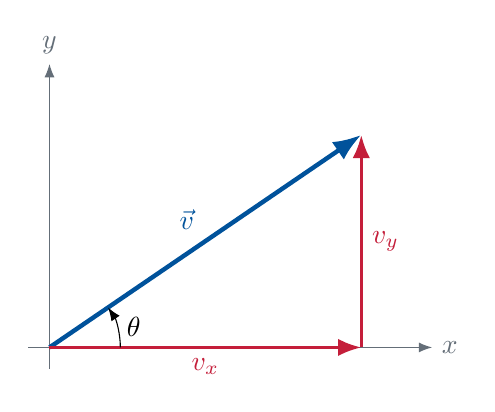
\begin{tikzpicture}[x=0.9cm,y=0.9cm,>=Latex]
      \draw[->,GraphGray] (-0.3,0)--(5.4,0) node[right]{$x$};
      \draw[->,GraphGray] (0,-0.3)--(0,4.0) node[above]{$y$};
      \draw[->,ultra thick,JapanBlue] (0,0)--(4.4,3.0) node[midway,above left]{$\vec v$};
      \draw[->,very thick,ChinaRed] (0,0)--(4.4,0) node[midway,below]{$v_x$};
      \draw[->,very thick,ChinaRed] (4.4,0)--(4.4,3.0) node[midway,right]{$v_y$};
      \draw[->] (1.0,0) arc[start angle=0,end angle=34.3,radius=1.0] node[midway,right]{$\theta$};
    \end{tikzpicture}
    \end{center}
  \end{columns}
\end{frame}

% 14
\begin{frame}{運動の分解（Decomposition）}
  \begin{columns}[T,onlytextwidth]
    \column{0.50\textwidth}
    \begin{block}{速度の成分}
      \[
        v_x=v\cos\theta,
        \qquad
        v_y=v\sin\theta
      \]
      斜向运动可以分别研究水平与竖直方向。
    \end{block}
    \begin{alertblock}{独立性}
      \begin{itemize}
        \item 两个方向使用同一个时间 $t$
        \item 一个方向的运动不会“消耗”另一个方向的速度
        \item 分解是分析方法，实际物体只有一条轨迹
      \end{itemize}
    \end{alertblock}

    \column{0.46\textwidth}
    \begin{center}
    \begin{tikzpicture}[x=0.9cm,y=0.9cm,>=Latex]
      \coordinate (O) at (0,0);
      \coordinate (P) at (4.5,2.8);
      \draw[->,ultra thick,JapanBlue] (O)--(P) node[midway,above left]{$\vec v$};
      \draw[->,very thick,ChinaRed] (O)--(4.5,0) node[midway,below]{$\vec v_x$};
      \draw[->,very thick,ChinaRed] (4.5,0)--(P) node[midway,right]{$\vec v_y$};
      \draw[dashed,GraphGray] (P)--(0,2.8);
      \draw[->] (1,0) arc[start angle=0,end angle=31.9,radius=1] node[midway,right]{$\theta$};
      \node[below] at (2.2,-0.7) {水平 + 竖直};
    \end{tikzpicture}
    \end{center}
  \end{columns}
\end{frame}

% 15
\begin{frame}{投射運動の分解}
  \begin{columns}[T,onlytextwidth]
    \column{0.55\textwidth}
    \begin{center}
    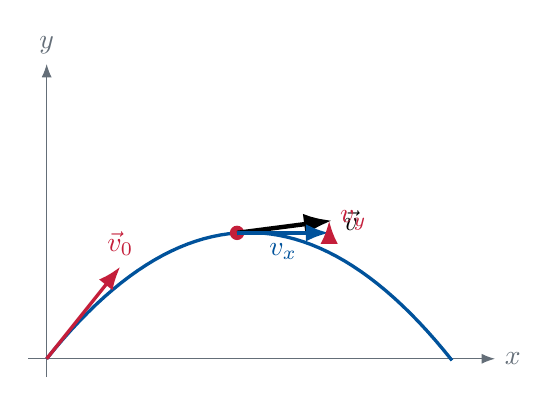
\begin{tikzpicture}[x=0.78cm,y=0.78cm,>=Latex]
      \draw[->,GraphGray] (-0.3,0)--(7.3,0) node[right]{$x$};
      \draw[->,GraphGray] (0,-0.3)--(0,4.8) node[above]{$y$};
      \draw[very thick,JapanBlue,domain=0:6.6,samples=50]
        plot (\x,{1.25*\x-0.19*\x*\x});
      \coordinate (P) at (3.1,2.05);
      \fill[ChinaRed] (P) circle (2.6pt);
      \draw[->,ultra thick,black] (P)--($(P)+(1.55,0.2)$) node[right]{$\vec v$};
      \draw[->,very thick,JapanBlue] (P)--($(P)+(1.5,0)$) node[midway,below]{$v_x$};
      \draw[->,very thick,ChinaRed] ($(P)+(1.5,0)$)--($(P)+(1.5,0.2)$) node[right]{$v_y$};
      \draw[->,very thick,ChinaRed] (0,0)--(1.2,1.5) node[above]{$\vec v_0$};
    \end{tikzpicture}
    \end{center}

    \column{0.41\textwidth}
    \begin{block}{水平方向}
      \[
        x=v_0\cos\theta\,t,
        \qquad v_x=v_0\cos\theta
      \]
    \end{block}
    \begin{alertblock}{鉛直方向}
      \[
        y=v_0\sin\theta\,t-\frac12gt^2
      \]
      \[
        v_y=v_0\sin\theta-gt
      \]
    \end{alertblock}
  \end{columns}
\end{frame}

% 16
\begin{frame}{運動の合成（Composition）}
  \begin{columns}[T,onlytextwidth]
    \column{0.52\textwidth}
    \begin{center}
    \begin{tikzpicture}[x=0.9cm,y=0.9cm,>=Latex]
      \coordinate (O) at (0,0);
      \coordinate (X) at (4.3,0);
      \coordinate (Y) at (0,2.8);
      \coordinate (R) at (4.3,2.8);
      \draw[->,very thick,JapanBlue] (O)--(X) node[midway,below]{$\vec v_x$};
      \draw[->,very thick,ChinaRed] (O)--(Y) node[midway,left]{$\vec v_y$};
      \draw[dashed,JapanBlue] (Y)--(R);
      \draw[dashed,ChinaRed] (X)--(R);
      \draw[->,ultra thick,black] (O)--(R) node[midway,above left]{$\vec v$};
      \node[below] at (2.2,-0.7) {平行四辺形法};
    \end{tikzpicture}
    \end{center}

    \column{0.44\textwidth}
    \begin{block}{合速度}
      \[
        \vec v=\vec v_x+\vec v_y
      \]
      两个互相垂直的分量合成为实际速度。
    \end{block}
    \begin{alertblock}{大きさ}
      \[
        v=\sqrt{v_x^2+v_y^2}
      \]
      \[
        \tan\theta=\frac{v_y}{v_x}
      \]
    \end{alertblock}
  \end{columns}
\end{frame}

% 17
\begin{frame}{相対速度：船が川を渡る}
  \begin{columns}[T,onlytextwidth]
    \column{0.55\textwidth}
    \begin{center}
    \begin{tikzpicture}[x=0.78cm,y=0.78cm,>=Latex]
      \fill[SoftBlue] (-0.3,-0.4) rectangle (6.8,4.5);
      \draw[very thick,JapanBlue] (-0.3,-0.4)--(6.8,-0.4);
      \draw[very thick,JapanBlue] (-0.3,4.5)--(6.8,4.5);
      \foreach \y in {0.3,1.3,2.3,3.3}{
        \draw[->,JapanBlue!70] (0.2,\y)--(1.2,\y);
      }
      \coordinate (O) at (1.4,0.4);
      \draw[->,ultra thick,ChinaRed] (O)--(1.4,3.8) node[midway,left]{$\vec v_{\text{船/水}}$};
      \draw[->,ultra thick,JapanBlue] (O)--(4.5,0.4) node[midway,below]{$\vec v_{\text{水/地}}$};
      \draw[->,ultra thick,black] (O)--(4.5,3.8) node[midway,above left]{$\vec v_{\text{船/地}}$};
      \draw[dashed] (1.4,3.8)--(4.5,3.8)--(4.5,0.4);
      \node at (5.6,2.2) {实际航线};
    \end{tikzpicture}
    \end{center}

    \column{0.41\textwidth}
    \begin{block}{速度の合成}
      \[
        \vec v_{\text{船/地}}
        =\vec v_{\text{船/水}}
        +\vec v_{\text{水/地}}
      \]
    \end{block}
    \begin{alertblock}{相対速度}
      \[
        \vec v_{A/B}=\vec v_A-\vec v_B
      \]
      “A 相对于 B 的速度”等于 A、B 对同一参考系速度之差。
    \end{alertblock}
  \end{columns}
\end{frame}

\section{練習と総括}

% 18
\begin{frame}{練習問題 I：位置と速度}
  \begin{enumerate}
    \item 某人从 $x=2\,\mathrm m$ 走到 $x=12\,\mathrm m$，再返回 $x=5\,\mathrm m$。求移动距离和位移。
    \vspace{0.35em}
    \item 汽车在 $8\,\mathrm s$ 内向东移动 $160\,\mathrm m$。求平均速率与平均速度。
    \vspace{0.35em}
    \item 已知
      \[
        x(t)=2t^2-3t+1,
      \]
      求 $v(t)$ 与 $t=2\,\mathrm s$ 时的速度。
    \item 两物体满足 $x_A=4t$、$x_B=30-2t$。求相遇时间与位置。
  \end{enumerate}
  \begin{alertblock}{ヒント}
    位移只看起点和终点；瞬时速度用 $v=\dd x/\dd t$；相遇时 $x_A=x_B$。
  \end{alertblock}
\end{frame}

% 19
\begin{frame}{練習問題 II：分解と合成}
  \begin{enumerate}
    \item 大小为 $20\,\mathrm{m/s}$ 的速度与水平线成 $30^\circ$。求 $v_x$、$v_y$。
    \vspace{0.4em}
    \item 已知 $v_x=6\,\mathrm{m/s}$、$v_y=8\,\mathrm{m/s}$。求合速度的大小与方向。
    \vspace{0.4em}
    \item 船相对水以 $3\,\mathrm{m/s}$ 垂直河岸航行，水流速度为 $4\,\mathrm{m/s}$。求船相对地面的速度大小。
    \vspace{0.4em}
    \item 为什么斜方投射在最高点仍然具有速度？请用速度分量说明。
  \end{enumerate}
  \begin{alertblock}{ヒント}
    \[
      v_x=v\cos\theta,\qquad v_y=v\sin\theta,
      \qquad v=\sqrt{v_x^2+v_y^2}.
    \]
  \end{alertblock}
\end{frame}

% 20
\begin{frame}{解答・総括}
  \small
  \begin{columns}[T,onlytextwidth]
    \column{0.48\textwidth}
    \begin{block}{練習 I}
      \begin{enumerate}
        \item 距離 $17\,\mathrm m$，変位 $+3\,\mathrm m$
        \item $20\,\mathrm{m/s}$，向东 $20\,\mathrm{m/s}$
        \item $v=4t-3$，$v(2)=5\,\mathrm{m/s}$
        \item $t=5\,\mathrm s$，$x=20\,\mathrm m$
      \end{enumerate}
    \end{block}
    \begin{alertblock}{基本公式}
      \[
        \Delta x=x_2-x_1,qquad
        v=\frac{\dd x}{\dd t}
      \]
    \end{alertblock}

    \column{0.48\textwidth}
    \begin{block}{練習 II}
      \begin{enumerate}
        \item $(v_x,v_y)=(10\sqrt3,10)\,\mathrm{m/s}$
        \item $v=10\,\mathrm{m/s}$，$\theta\approx53^\circ$
        \item $v=5\,\mathrm{m/s}$
        \item 最高点 $v_y=0$，但 $v_x\neq0$
      \end{enumerate}
    \end{block}
    \begin{alertblock}{合成公式}
      \[
        \vec v=\vec v_x+\vec v_y,qquad
        v=\sqrt{v_x^2+v_y^2}
      \]
    \end{alertblock}
  \end{columns}
\end{frame}

% 21
\begin{frame}{参考文献}
  \small
  \begin{columns}[T,onlytextwidth]
    \column{0.48\textwidth}
    \begin{block}{1\quad EJU 公式資料}
      \textbf{日本学生支援機構（JASSO）}\par
      \vspace{0.2em}
      2026年度 日本留学試験\par
      \jp{物理シラバス}\par
      \vspace{0.3em}
      {\scriptsize
      \href{https://www.jasso.go.jp/ryugaku/eju/examinee/syllabus/science_phy.html}
      {\color{JapanBlue}\underline{JASSO 公式ページを開く}}}
    \end{block}
    \begin{alertblock}{2\quad 日本語の物理用語}
      文部科学省 高等学校学習指導要領\par
      \emph{物理基礎・物理}
    \end{alertblock}

    \column{0.48\textwidth}
    \begin{block}{3\quad 基礎物理}
      \textbf{S. J. Ling, W. Moebs, J. Sanny}\par
      \emph{University Physics, Volume 1}\par
      OpenStax, Rice University, 2022.\par
      \vspace{0.3em}
      {\scriptsize
      \href{https://openstax.org/details/books/university-physics-volume-1}
      {\color{JapanBlue}\underline{OpenStax で読む}}}
    \end{block}
    \begin{alertblock}{4\quad 発展参考}
      \textbf{R. A. Serway, J. W. Jewett}\par
      \emph{Physics for Scientists and Engineers}\par
      10th ed., Cengage Learning, 2018.
    \end{alertblock}
  \end{columns}
  \vfill
  \centering
  {\footnotesize 日语概念用于应试，中文解释用于理解，英文术语用于补充。}
\end{frame}

\end{document}
